\documentclass[12pt]{article}

\usepackage{lmodern}
\usepackage[T1]{fontenc}
\usepackage[utf8]{inputenc}
\usepackage[spanish, activeacute]{babel}
\usepackage{listings}
\usepackage{enumitem}
\usepackage{graphicx}
\usepackage{float}
\usepackage[hidelinks]{hyperref}
\usepackage{xcolor}

\definecolor{mygreen}{rgb}{0,0.6,0}
\definecolor{mygray}{rgb}{0.8,0.8,0.8}
\definecolor{mymauve}{rgb}{0.58,0,0.82}
\lstset{
backgroundcolor=\color{white},
basicstyle=\ttfamily,
breakatwhitespace=false,
captionpos=b,
commentstyle=\color{mygreen},
deletekeywords={...},
escapeinside={\%*}{*)},
extendedchars=true,
keepspaces=true,
keywordstyle=\color{blue},
language=Octave,
morekeywords={*,...},
numbers=left,
numbersep=5pt,
numberstyle=\tiny\color{black},
showspaces=false,
showstringspaces=false,
showtabs=false,
stepnumber=1,
stringstyle=\color{mymauve},
tabsize=2,
}

\graphicspath {{ assets/images/ }}

\title{Práctica 06 - Web Server}
\author{
    Wilson Aguilar \\
    \textsc{Plataformas Web}
}

\begin{document}

\maketitle

\section{Configuraciones iniciales}

En esta práctica nos centraremos en la creación de un sitio web dinámico haciendo uso de nodejs y algunas librerias que nos ofrece esta tecnología.

Primero creamos un nuevo proyecto de node con el comando:

\begin{lstlisting}[numbers=none]
  npm init -y
\end{lstlisting}

En comparación con otros lenguajes de programación como Java o PHP donde tenemos que hacer uso de algún programa externo que haga de servidor para que pueda servir nuestros archivos, en node js lo podemos hacer de una manera mucho mas sencilla. NodeJs nos da la posibilidad de crear el servidor mediante la programación de una manera sencilla, para ello tenemos el módulo nativo http que trae node y otra es hacer uso de alguna libreria que nos fácilite la creación del servidor.

\subsection{Módulo http de node}

El módulo http de node nos permite levantar un servidor web con varias lineas de código. Podemos enviar al cliente html, archivos, etc.

Para ello empezamos creando un archivo con la siguiente configuración:

\begin{figure}[H]
  \centering
  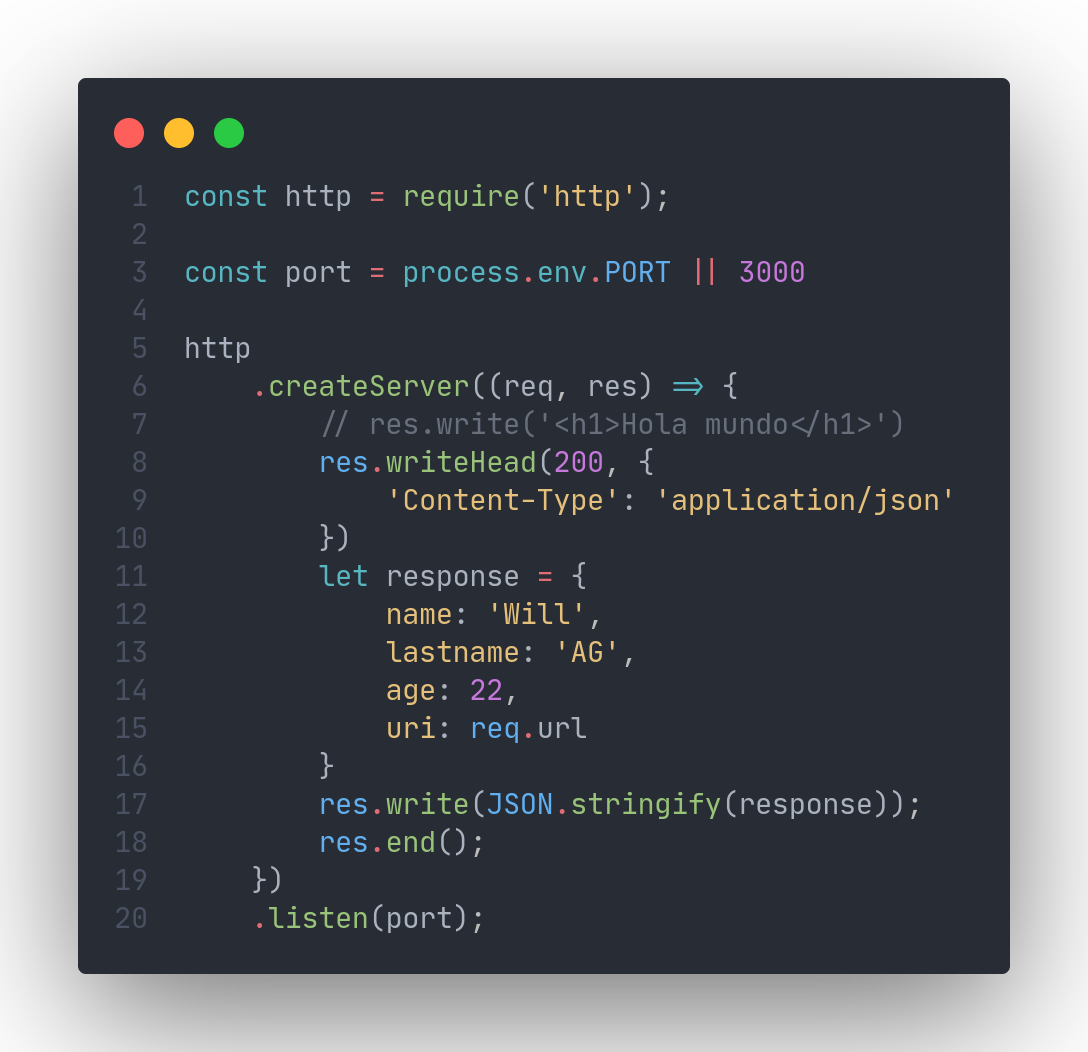
\includegraphics[scale=.35]{assets/images/basic-server.png}
  \caption{Servidor web con el modulo http de node}
\end{figure}

En este caso lo que mandamos al cliente son datos con formato Json. Observamos que la creación del servidor es muy sencilla pero el problema viene al momento de manejar rutas y tratar de tener contenido dinámico. Para ello tenemos muchas librerias o paquetes que nos facilitan el trabajo, entre ellas, algunas librerias famosas son:

\begin{itemize}
  \item Express
  \item Nest
  \item Koa
\end{itemize}

\subsection{Express}

Express es probablemente la libreria mas famosa para la creación de aplicaciones web. Esta libreria nos hace el trabajo mucho mas fácil debido a que tiene varias cosas ya configuradas y no debemos preocuparnos por resolver problemas muy triviales.

Express esta basado en el módulo http nativo de node, por lo que se lo puede integrar con este fácilmente. Para crear el servidor creamos un archivo server.js con el siguiente código.

\begin{figure}[H]
  \centering
  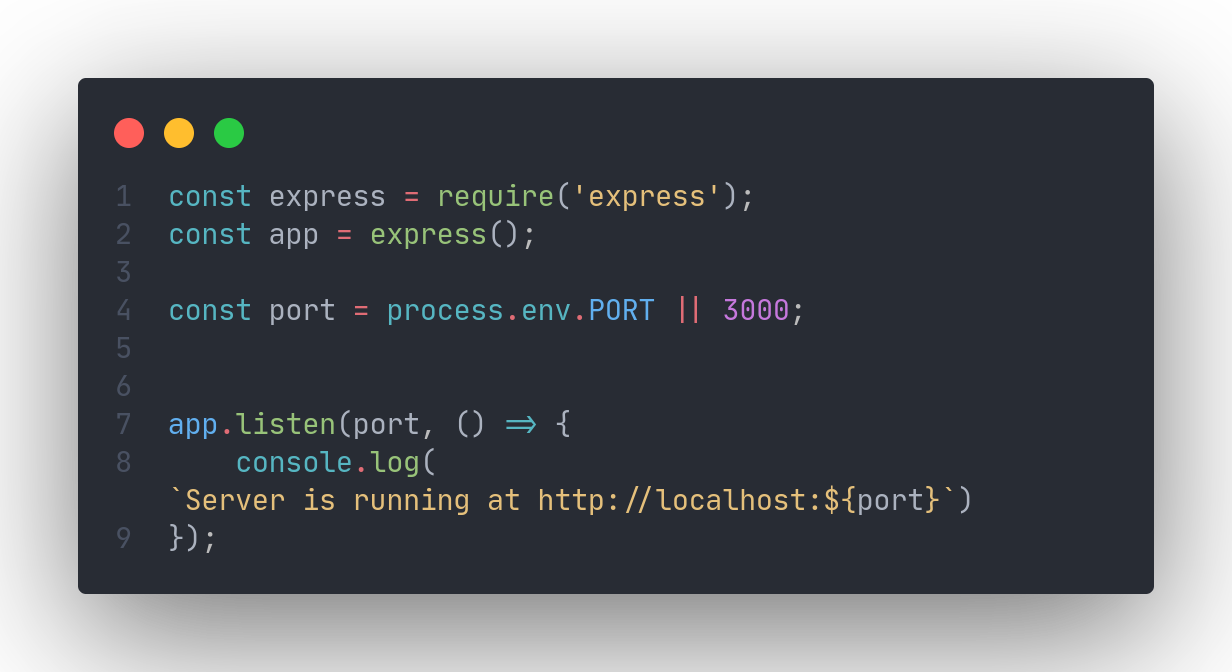
\includegraphics[scale=.3]{assets/images/express-server.png}
  \caption{Servidor con express.}
\end{figure}

En este punto tenemos nuestro servidor corriendo en el puerto definido (en este caso 300).

\section{Contenido estático}

Ahora lo que haremos es crear algunas páginas web en html para que nuestro servidor pueda enviar esas páginas cuando algún cliente lo solicita. La manera mas común de hacerlo es crear un directorio con los archivos que se van a visualizar, y los recursos que esta va a utilizar.
Para ello en la raíz de nuestro proyecto creamos un directorio publico donde van a estar todos los archivos que va a poder ser accedidos desde la parte del cliente.

\begin{figure}[H]
  \centering
  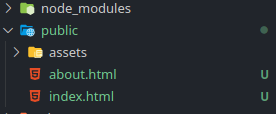
\includegraphics{assets/images/static.png}
  \caption{Directorio con archivos publicos.}
\end{figure}

En esta carpeta public van a estar los archivos html y recursos que va a mostrar el servidor. Después de crear este directorio le debemos decir a express el path completo donde se encuentra el directorio. Nos dirigimos al archivo principal y agregamos lo siguiente:

\begin{figure}[H]
  \centering
  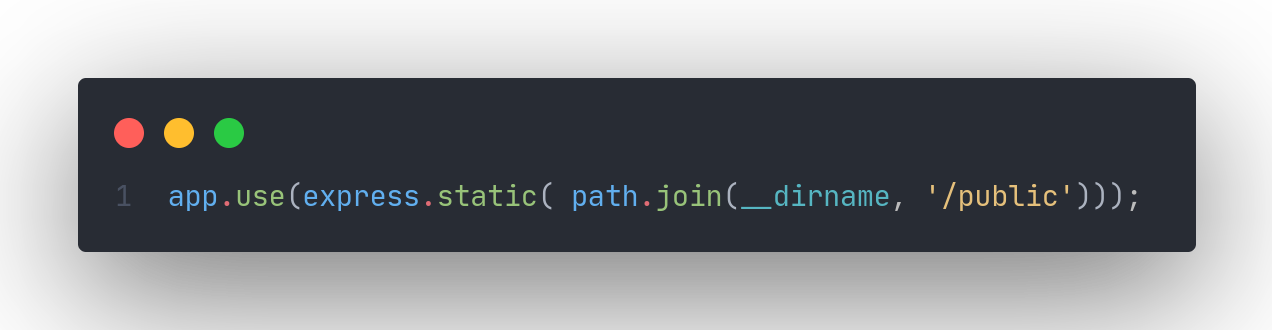
\includegraphics[scale=.3]{assets/images/static-folder.png}
  \caption{Definiendo carpeta publica.}
\end{figure}


\section{Motor de platillas}

Realizar un sitio web haciendo uso solo de html puede ser muy tedioso ya que por cada página tenemos que repetir la misma estructura, es decir vamos a tener que escribir lo mismo una y otra vez. Los motores de plantillas nos permiten la reutilización del código html ya escrito anteriormete y dividirlos como plantillas que podemos reutilizar cuando sea necesario, esto nos ayuda a escribir solo el contenido necesario.

El motor de plantillas utlizado en la practica es handle bars, pero tambien existen otros que podriamos utilizar como son:

\begin{itemize}
  \item Pug
  \item Ejs
\end{itemize}

\subsection{Handlebars}

Handlebars es un motor de plantillas que nos permite hace mas dinámicao el sitio web haciendo uso de variables, funciones dentro del html. Para hacer uso de handlebars en nuestro proyecto de node primero lo instalamos haciendo uso de:

\begin{lstlisting}[numbers=none]
  npm install hbs
\end{lstlisting}

Ahora en nuestro archivo principal importamos la libreria y realizamos la siguiente configuración.

\begin{figure}[H]
  \centering
  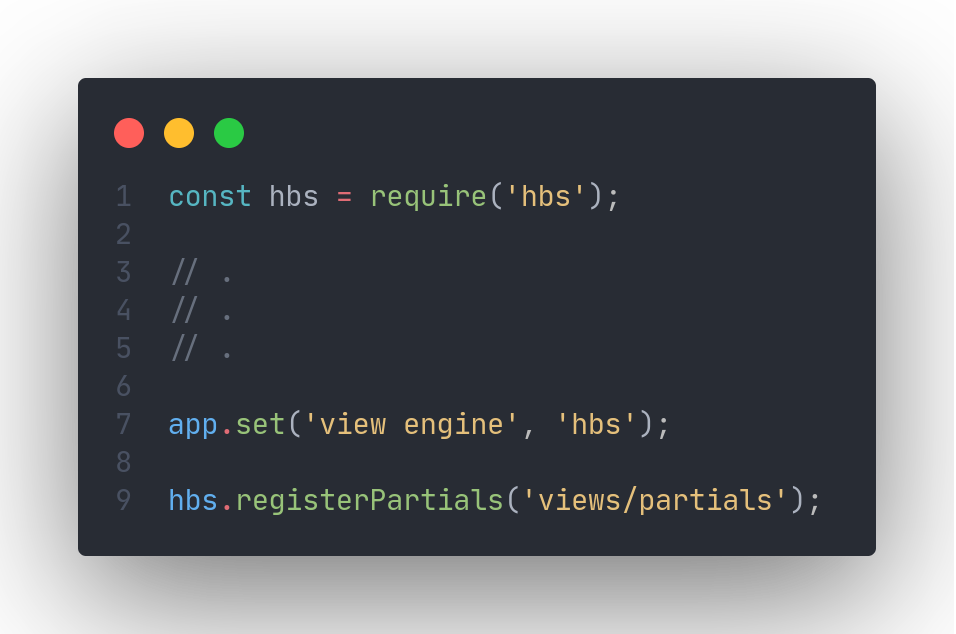
\includegraphics[scale=.4]{assets/images/handlebars-code.png}
  \caption{Configuración de handlebars.}
\end{figure}

En esta configuración lo que decimos es que hbs va a ser el motor de vistas. También utilizamos hbs para registrar los partial.

Para poder hacer uso de handlebars creamos una carpeta que se llame views y dentro de ella iran archivos con la extension.hbs que usen html como si se tratara de cualquier otra página.

\begin{figure}[H]
  \centering
  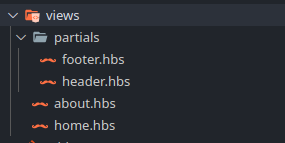
\includegraphics[]{assets/images/partials.png}
  \caption{Configuración de handlebars.}
\end{figure}

\subsection{Partials}

Los partials vienen a ser nuestras plantillas, el código html que escribimos y que puede ser reutilizado. En este caso tenemos 2 partials el header y el footer ya que se van a repetir en todas las páginas que tenemos.

Para registrar los partials en nuestro archivo principal usamos el siguiente comando:

\begin{lstlisting}[numbers=none]
  hbs.registerPartials('views/partials');
\end{lstlisting}

Para usar los partils lo hacemos de la siguiente manera:

\begin{figure}[H]
  \centering
  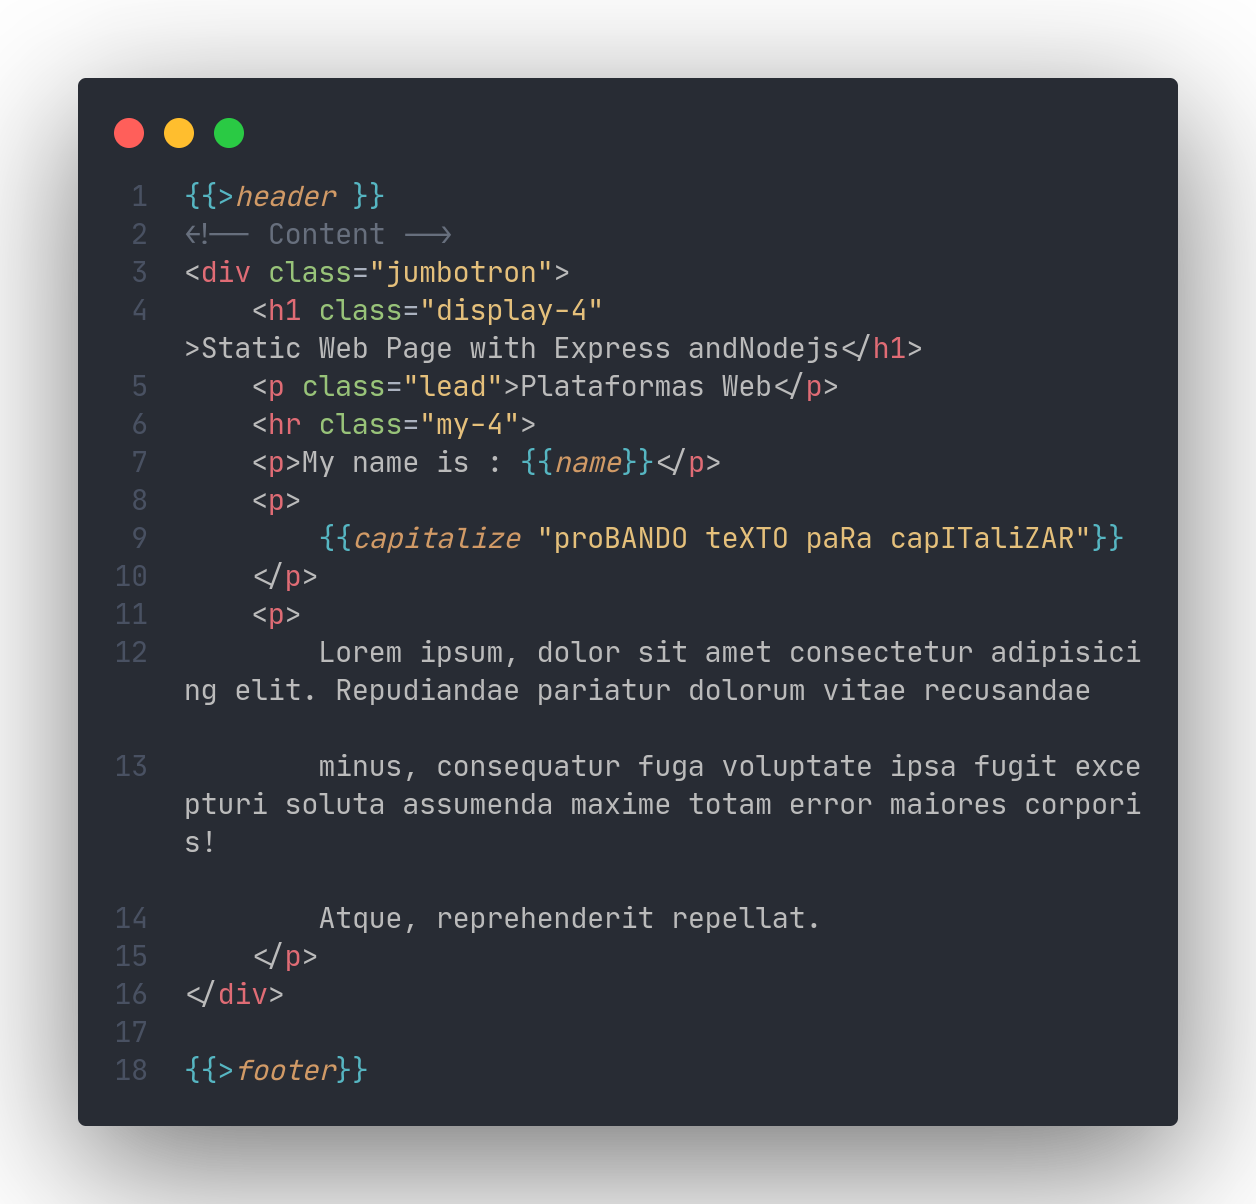
\includegraphics[scale=.3]{assets/images/partial-use.png}
  \caption{Uso de partials}
\end{figure}

Simplemente usamos \{> partial \}. Y en esa sección se agregara el código que tenemos en nuestro partial.

\subsection{Helpers}

Los helpers son funciones que podemos llamar directamente desde los templates, es decir podemos llamar una funcion sencilla que nos permita capitalizar un string u obtener el año actual.

Para crear los helpers simplemente creamos un archivo aparte con la siguiente configuración:

\begin{figure}[H]
  \centering
  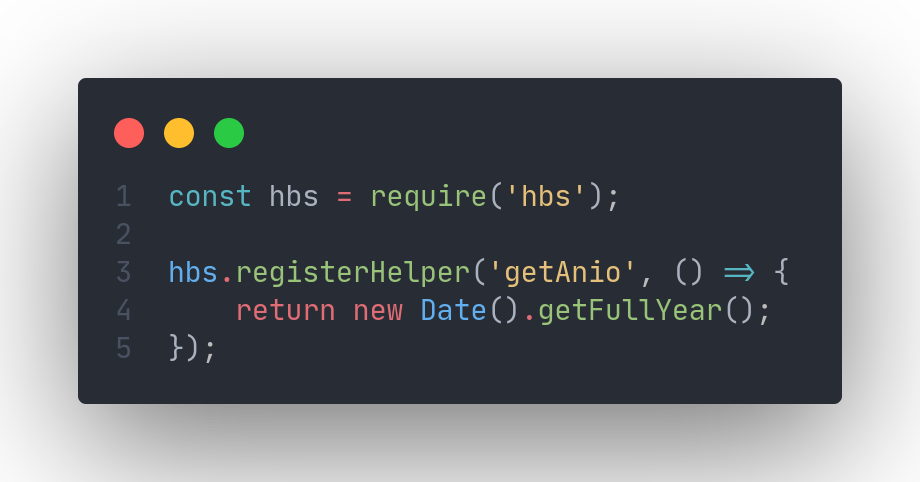
\includegraphics[scale=.4]{assets/images/helpers.png}
  \caption{Registro de nuevos helpers.}
\end{figure}

Para que los helpers queden completamente registrados, simplemente hacemos un \lstinline{require()} en el archivo principal, esto ayuda a que el archivo con las configuraciones cargue desde el principal.

Para usarlo simplemente entre llaves ponemos el nombre de la función. Por ejemplo \{> capitalize \}

\begin{figure}[H]
  \centering
  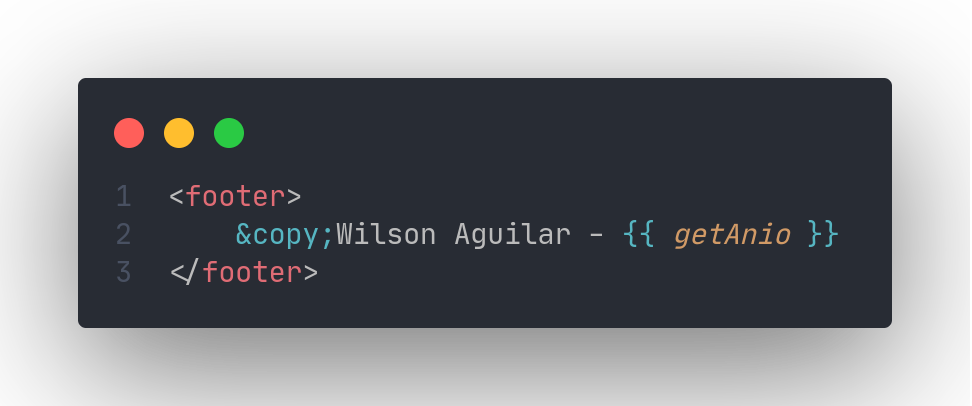
\includegraphics[scale=.4]{assets/images/helper-use.png}
  \caption{Uso de helpers.}
\end{figure}

\section{Subiendo a producción}

Para subir nuestra aplicación a internet vamos a usar la plataforma heroku, ya que es un servicio muy sencillo de usar.

Primero nos creamos una cuenta en heroku y después creamos una aplicación dentro de heroku.

Con la aplicación lista nos dirigimos a nustro proyecto e inicializamos un repositorio de git.

\begin{lstlisting}[numbers=none]
  git init
  git commit -m "first commit"
\end{lstlisting}

Ahora lo que hacemos es iniciar sesion con el heroku CLI, para ello ejecutamos el comando \lstinline{heroku login}. Nos llevará a una ventana del navegador para iniciar sesion.

Después agregamos el repositorio remoto de heroku a nuestro repositorio local para posteriormente subirlo ahi. Ejecutamos:

\begin{lstlisting}[numbers=none]
  heroku git:remote -a nombre-aplicacion-heroku
  git push -a heroku master
\end{lstlisting}

Con esto ya tendremos nuestro proyecto subido a heroku. ahora simplemente abrimos la url de nuestra aplicación en heroku o escribimos es comando \lstinline{heroku open} para abrir en una pestaña del navegador.

\begin{figure}[H]
  \centering
  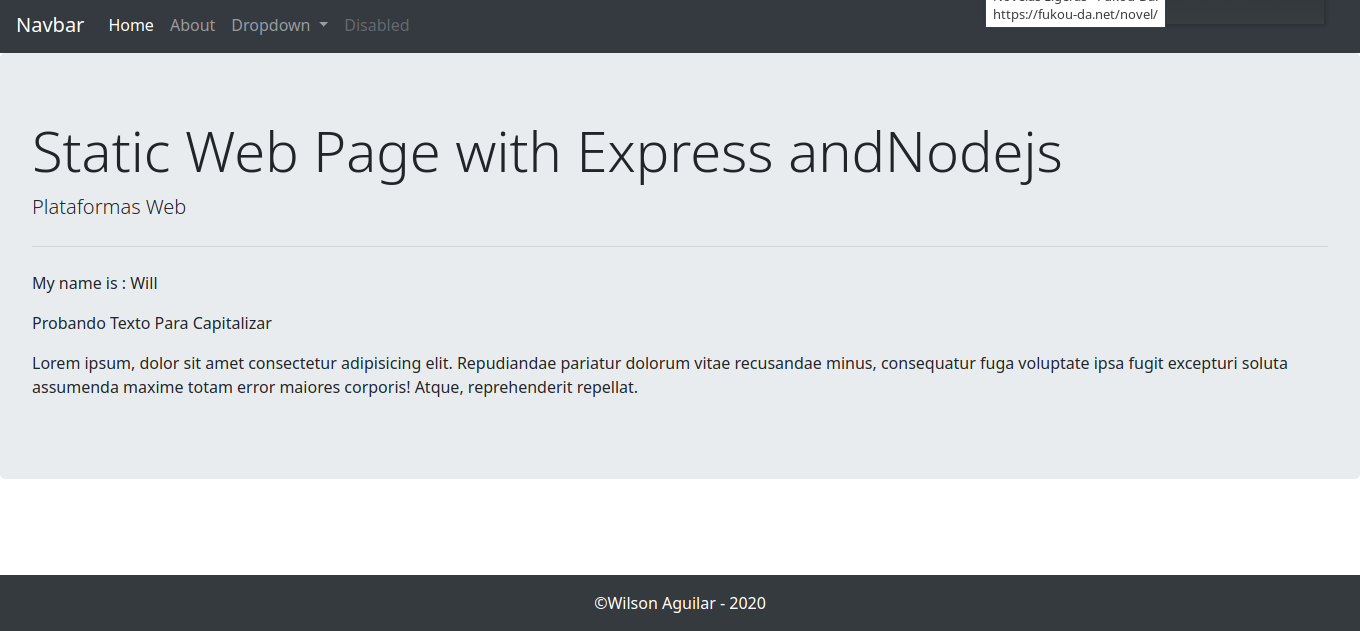
\includegraphics[scale=.35]{assets/images/web.png}
  \caption{Sitio web desplegado a heroku.}
\end{figure}

\section{Repositorio en Github}

El repositorio se encuentra en el siguiente enlace:

\url{https://github.com/WilsonAG/plataformas-web/tree/master/node/06-webserver}

\end{document}